\chapter{Лабораторная работа №2 \\
Расчёт и моделирование двухшлейфного направленного ответвителя}

Цель работы: ознакомиться с расчётом и моделированием двухшлейфного направленного ответвителя в среде Keysight Advanced Design System (ADS).

Используемое оборудование или ПО: Keysight Advanced Design System 2020 upd1.

\section{Техническое задание}

Рассчитать и спроектировать двухшлейфный направленный ответвитель на входную частоту $F_c = 7 \text{~ГГц}$.
Провести её настройку и исследование на схемном и топологическом уровнях.

В качестве подложки использовать Arlon AD255C с относительной диэлектрической проницаемостью $\epsilon = 2.55$, тангенсом угла диэлектрических потерь $\tg{\delta} = 0.0013$, толщиной диэлектрика $H = 0.508 \text{~мм}$ и толщиной металлизации $T = 35 \text{~мкм}$.

\section{Выполнение работы}

\subsection{Создание подложки}

В первую очередь зададим параметры подложки. Для этого в главном окне перейдём по пути Options\textrightarrow Technology\textrightarrow Edit Stackup (tech.subst) и выберем пункт Create the master substrate from scratch.
В качестве шаблона используем 25milAlumina.
Параметры подложки возьмём из технического задания.
Результат представлен на рис. \ref{fig:branch_line_coupler_substrate}.

\begin{figure}
    \centering
    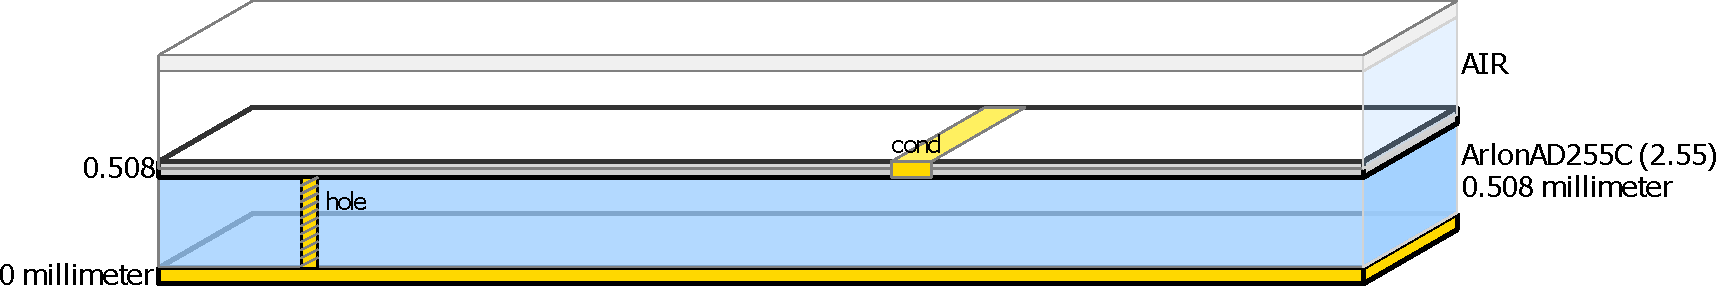
\includegraphics[width=0.9\textwidth]{branch_line_coupler_substrate.pdf}
    \caption{Подложка}
    \label{fig:branch_line_coupler_substrate}
\end{figure}

\subsection{Модель на идеальных линиях передачи}

Соберём моделируемую схему на идеальных линиях передачи (Рис. \ref{fig:branch_line_coupler_ideal_schematic}).

\begin{figure}[!ht]
    \centering
    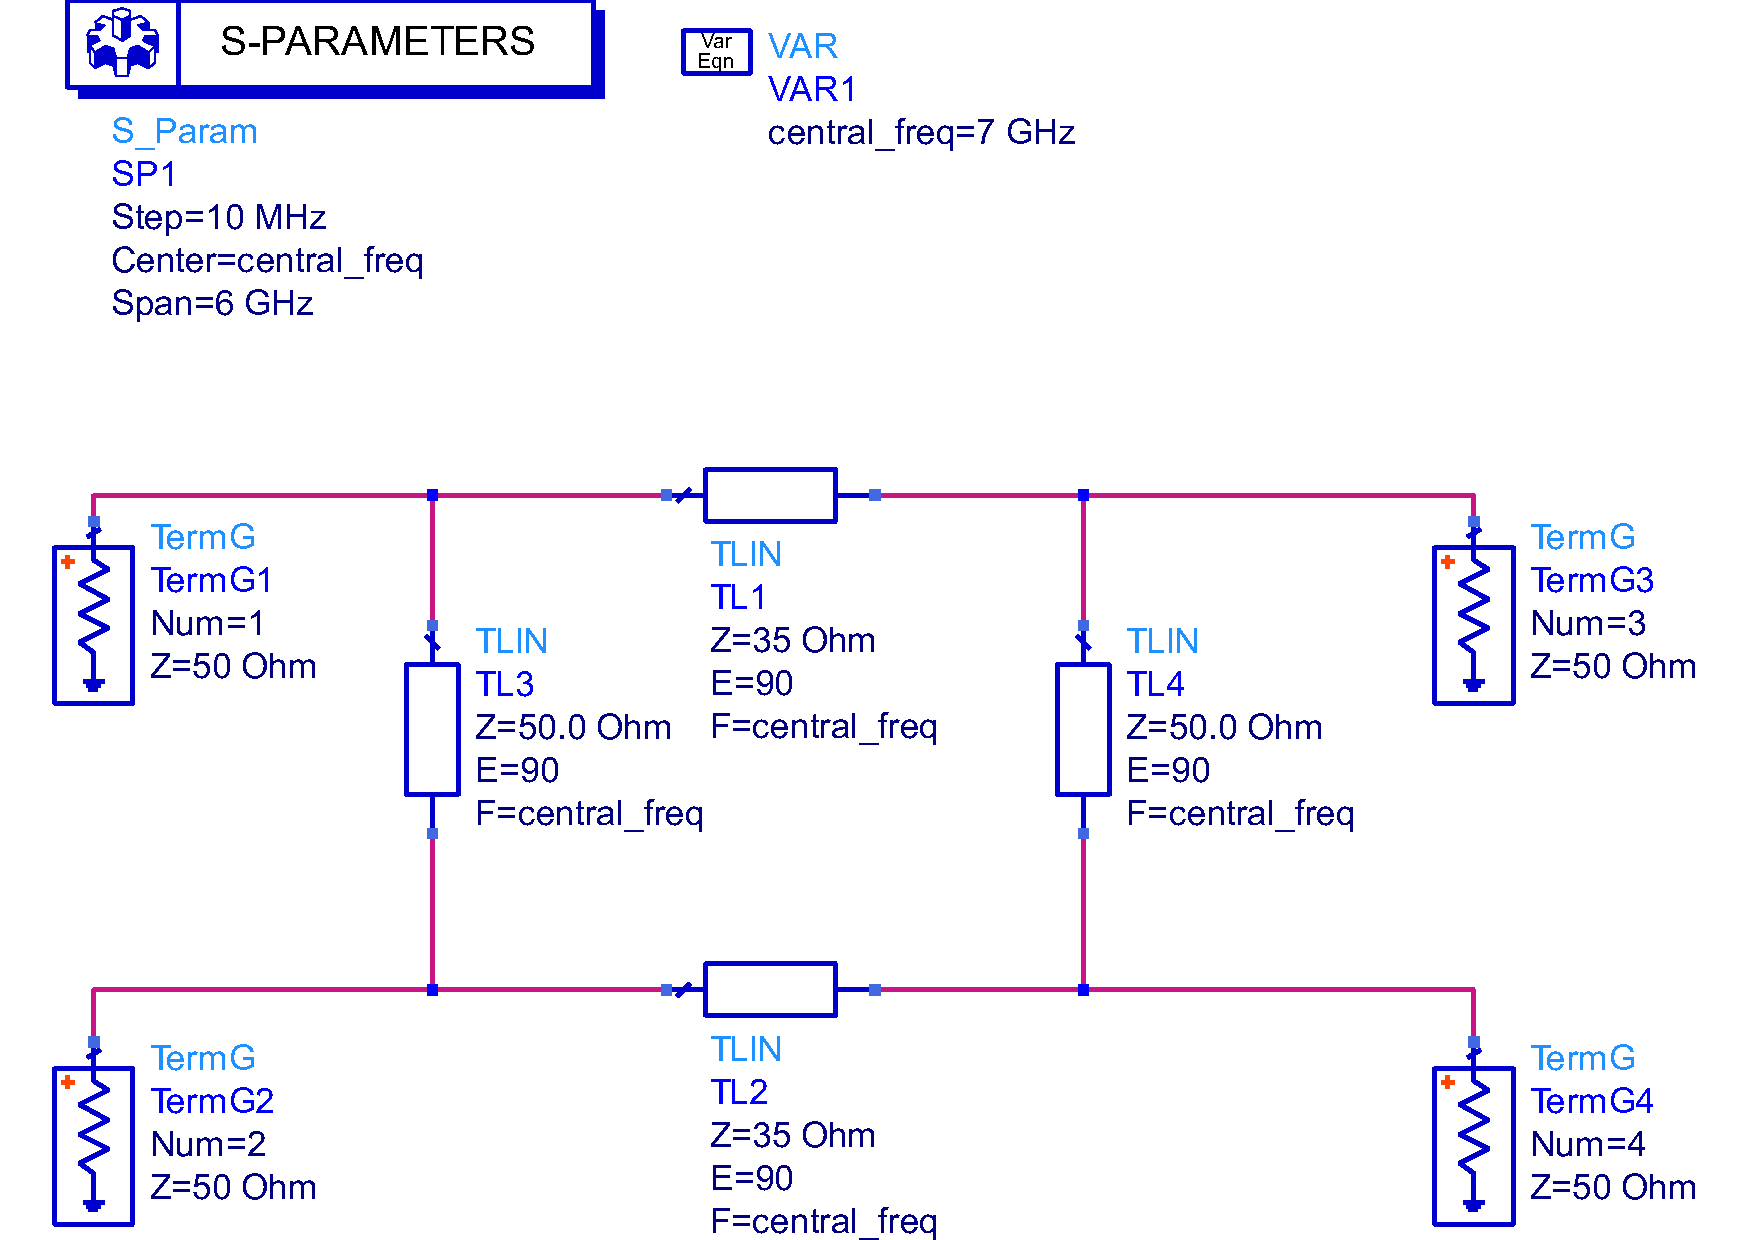
\includegraphics[width=0.8\textwidth]{branch_line_coupler_ideal_schematic.pdf}
    \caption{Моделируемая цепь на идеальных линиях передачи}
    \label{fig:branch_line_coupler_ideal_schematic}
\end{figure}

Результаты моделирования можно увидеть на рис. \ref{fig:branch_line_coupler_ideal_data_1_freq_response}.

\begin{figure}[!ht]
    \centering
    \begin{subfigure}[b]{0.45\textwidth}
        \centering
        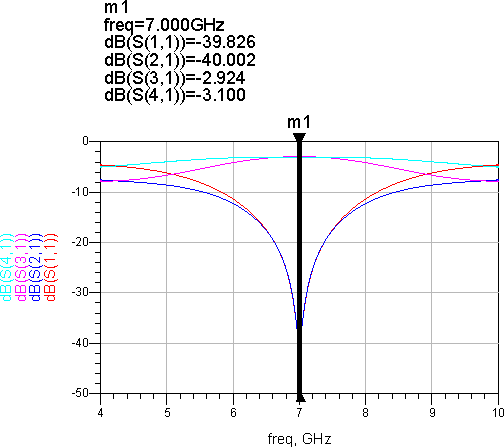
\includegraphics[width=\textwidth]{branch_line_coupler_ideal_data_1_freq_response.pdf}
        \caption{}
        \label{fig:branch_line_coupler_ideal_data_1_freq_response}
    \end{subfigure}
    \hfill
    \begin{subfigure}[b]{0.45\textwidth}
        \centering
        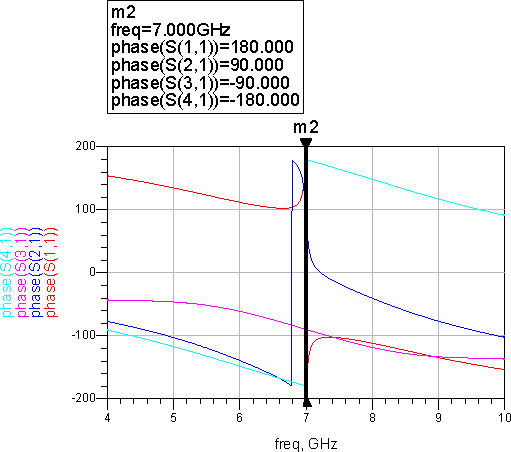
\includegraphics[width=\textwidth]{branch_line_coupler_ideal_data_1_phase_response.pdf}
        \caption{}
        \label{fig:branch_line_coupler_ideal_data_1_phase_response}
    \end{subfigure}
    \caption{
        a) АЧХ моделируемой цепи;
        б) ФЧХ моделируемой цепи
    }
    \label{fig:branch_line_coupler_ideal_data_display_1}
\end{figure}

Для более точной оценки результата дополнительно выведем идеальную теоретическую матрицу рассеяния и сравним с ней полученные результаты (Рис. \ref{fig:branch_line_coupler_ideal_data_1_smatrix}).
Также рассчитаем волновые сопротивления параллельного и последовательного участков относительно $Z_0 = 50 \text{~Ом}$ (Рис. \ref{fig:branch_line_coupler_ideal_data_1_impedances}).

\begin{figure}[!ht]
    \centering
    \begin{subfigure}[b]{0.7\textwidth}
        \centering
        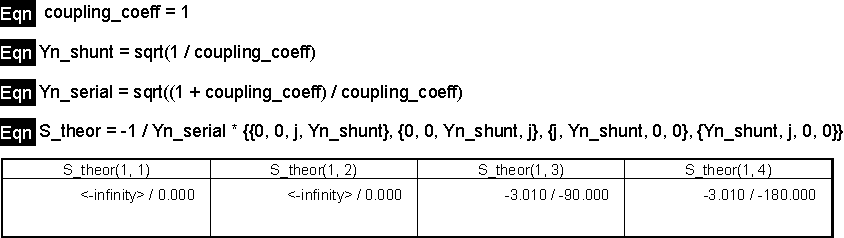
\includegraphics[width=\textwidth]{branch_line_coupler_ideal_data_1_smatrix.pdf}
        \caption{}
        \label{fig:branch_line_coupler_ideal_data_1_smatrix}
    \end{subfigure}
    \vfill
    \begin{subfigure}[b]{0.7\textwidth}
        \centering
        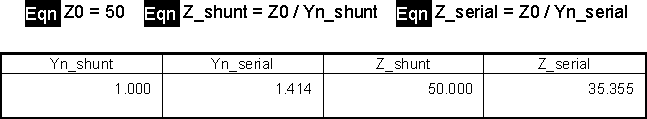
\includegraphics[width=\textwidth]{branch_line_coupler_ideal_data_1_impedances.pdf}
        \caption{}
        \label{fig:branch_line_coupler_ideal_data_1_impedances}
    \end{subfigure}
    \caption{
        a) Идеальная теоретическая матрица рассеяния;
        б) волновые сопротивления последовательного и параллельного участков
    }
    \label{fig:branch_line_coupler_ideal_data_display_2}
\end{figure}

\subsection{Модель на схемном уровне в микрополосковом исполнении}

Для расчёта геометрических размеров нескольких видов линий передач воспользуемся инструментом LineCalc, которую можно найти по пути Tools\textrightarrow LineCalc\textrightarrow Start LineCalc.

В подокне Substrate Parameters задаём параметры подложки из технического задания, в подокне Component Parameters задаём частоту из технического задания, а в подокне Electrical "--- импеданс и электрическую длину, для которых ведётся расчёт.
После этого, нажав кнопку Synthesize, получим в подокне Physical искомые геометрические размеры.

Расчитаем таким образом геометрические размеры параллельного и последовательного участков.
Получим $W_\text{shunt} = 1.383 \text{~мм}$, $L_\text{shunt} = 7.369 \text{~мм}$ и $W_\text{serial} = 2.330 \text{~мм}$, $L_\text{serial} = 7.222 \text{~мм}$ соответственно.

Построим моделируемую схему в микрополосковом исполнении (Рис. \ref{fig:branch_line_coupler_MLIN_schematic_1}).

\begin{figure}[!ht]
    \centering
    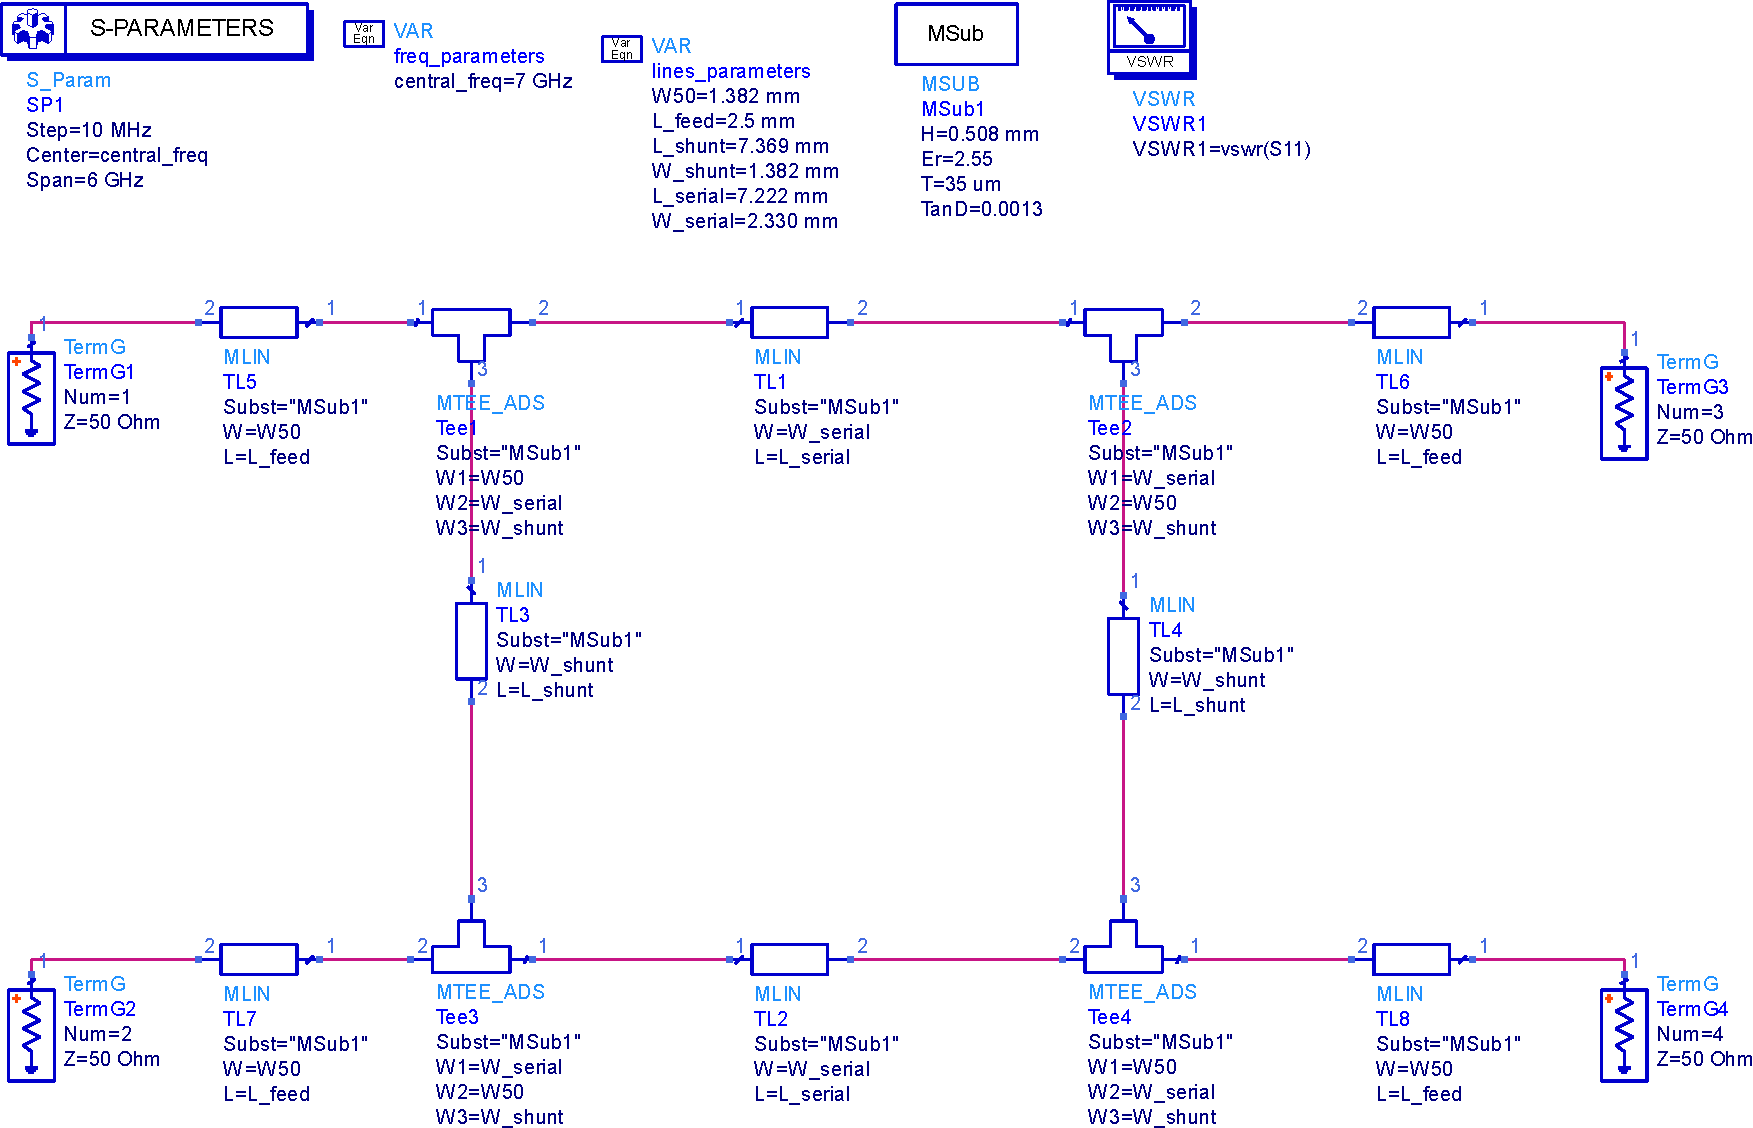
\includegraphics[width=0.8\textwidth]{branch_line_coupler_MLIN_schematic_1.pdf}
    \caption{Моделируемая схема в микрополосковом исполнении}
    \label{fig:branch_line_coupler_MLIN_schematic_1}
\end{figure}

Запустим расчёт и выведем АЧХ (Рис. \ref{fig:branch_line_coupler_MLIN_data_1_freq_response}).

\begin{figure}[!ht]
    \centering
    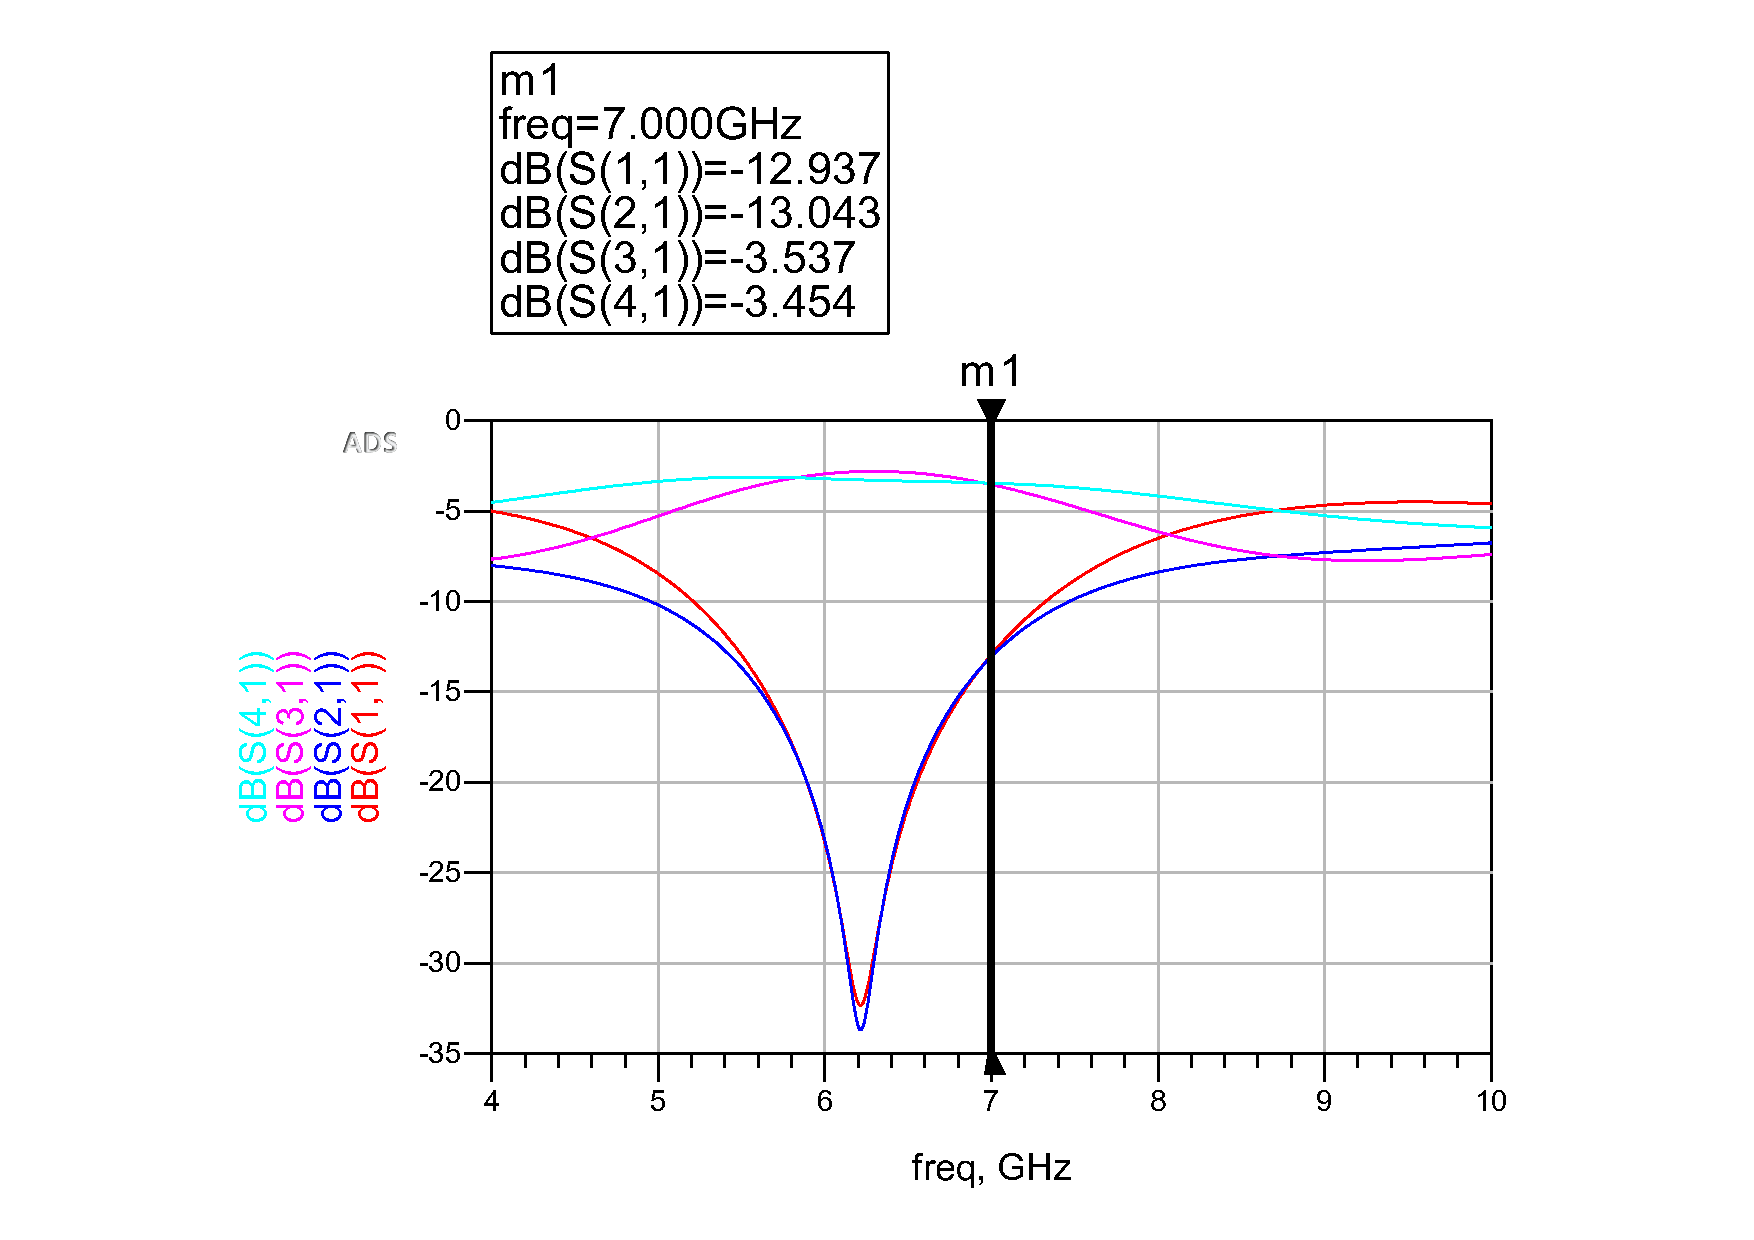
\includegraphics[width=\textwidth]{branch_line_coupler_MLIN_data_1_freq_response.pdf}
    \caption{АЧХ моделируемой схемы в микрополосковом исполнении}
    \label{fig:branch_line_coupler_MLIN_data_1_freq_response}
\end{figure}

Результаты показывают, что рабочая частота устройства уплыла вниз. Связано это с добавлением на схему тройников, в результате чего электрические длины шлейфов оказались больше, чем требуется.
Для того, чтобы исправить это, воспользуемся инструментом Tune.
В качестве изменяемых параметров укажем $L_\text{shunt}$, $W_\text{shunt}$, $L_\text{serial}$ и $W_\text{serial}$, для чего щёлкнем по ним левой кнопкой мыши.
Подберём оптимальный размер шага, после чего изменяя значения выбранных параметров с помощью слайдера, найдём такие, при которых обеспечивается наилучшее согласование.
В дополнение к этому поставим и следующие условия:
\begin{itemize}
    \item коэффициент отражения $dB(S_{11})$ и развязка $dB(S_{21})$ не должны превышать $-20 \text{~дБ}$ в диапазоне $(6.7 .. 7.3) \text{~ГГц}$;
    \item положение провалов коэффициента отражения $dB(S_{11})$ и развязки $dB(S_{21})$ как можно ближе к $7 \text{~ГГц}$;
    \item рабочее затухание $dB(S_{31})$ и переходное ослабление $dB(S_{41})$ не должны опускаться меньше $-3.5 \text{~дБ}$.
\end{itemize}
Для переноса получившихся значений на схему нажмём кнопку Update Schematic в окне Tune Parameters.

Итоговую схему можем увидеть на рис. \ref{fig:branch_line_coupler_MLIN_schematic_2}.

\begin{figure}
    \centering
    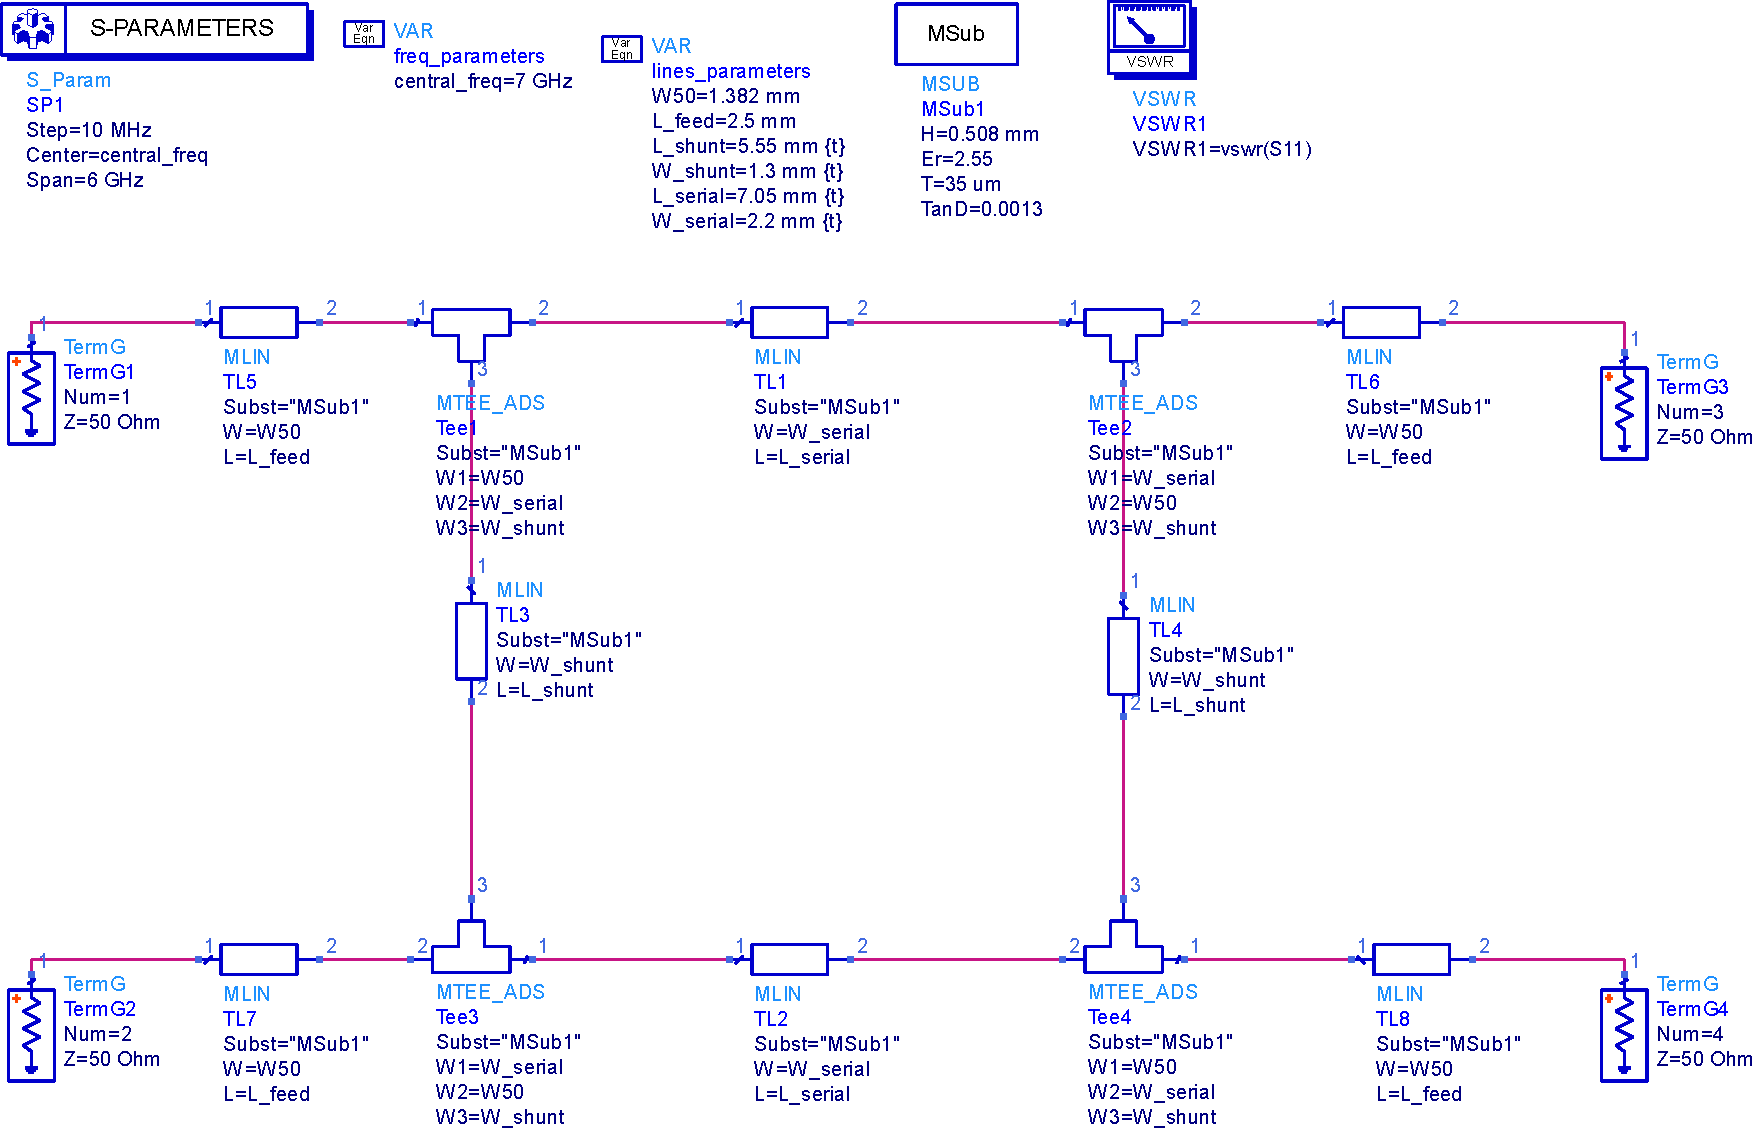
\includegraphics[width=0.6\textwidth]{branch_line_coupler_MLIN_schematic_2.pdf}
    \caption{Моделируемая схема в микрополосковом исполнении после применения инструмента Tune}
    \label{fig:branch_line_coupler_MLIN_schematic_2}
\end{figure}

Итоговые характеристики приобретут вид как на рис. \ref{fig:branch_line_coupler_MLIN_data_2}.

\begin{figure}[!ht]
    \centering
    \begin{subfigure}[b]{0.45\textwidth}
        \centering
        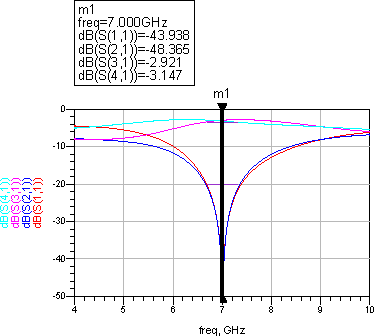
\includegraphics[width=\textwidth]{branch_line_coupler_MLIN_data_2_freq_response.pdf}
        \caption{}
        \label{fig:branch_line_coupler_MLIN_data_2_freq_response}
    \end{subfigure}
    \hfill
    \begin{subfigure}[b]{0.45\textwidth}
        \centering
        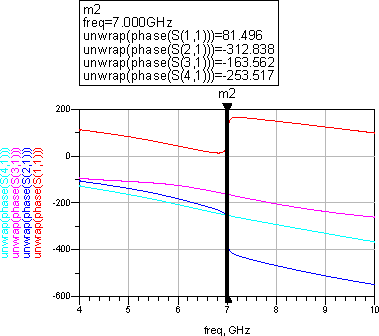
\includegraphics[width=\textwidth]{branch_line_coupler_MLIN_data_2_phase_response.pdf}
        \caption{}
        \label{fig:branch_line_coupler_MLIN_data_2_phase_response}
    \end{subfigure}
    \vfill
    \begin{subfigure}[b]{0.45\textwidth}
        \centering
        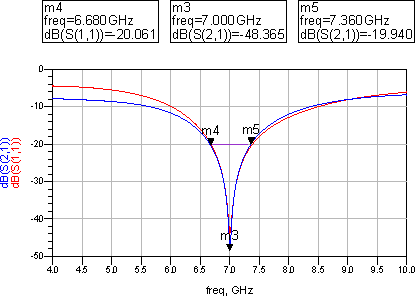
\includegraphics[width=\textwidth]{branch_line_coupler_MLIN_data_2_S11_S21_freq_response.pdf}
        \caption{}
        \label{fig:branch_line_coupler_MLIN_data_2_S11_S21_freq_response}
    \end{subfigure}
    \hfill
    \begin{subfigure}[b]{0.45\textwidth}
        \centering
        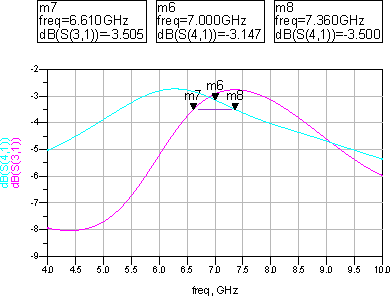
\includegraphics[width=\textwidth]{branch_line_coupler_MLIN_data_2_S31_S41_freq_response.pdf}
        \caption{}
        \label{fig:branch_line_coupler_MLIN_data_2_S31_S41_freq_response}
    \end{subfigure}
    \caption{
        Частотные характеристики моделируемой схемы в микрополосковом исполнении после применения инструмента Tune:
        a) АЧХ;
        б) ФЧХ;
        в) АЧХ коэффициента отражения и развязки;
        г) АЧХ рабочего затухания и переходного ослабления.
    }
    \label{fig:branch_line_coupler_MLIN_data_2}
\end{figure}

Неравномерность частотных характеристик в заданном диапазоне можно увидеть на рис. \ref{fig:branch_line_coupler_MLIN_data_2_response_ripple}.

\begin{figure}[!ht]
    \centering
    \begin{subfigure}[b]{0.6\textwidth}
        \centering
        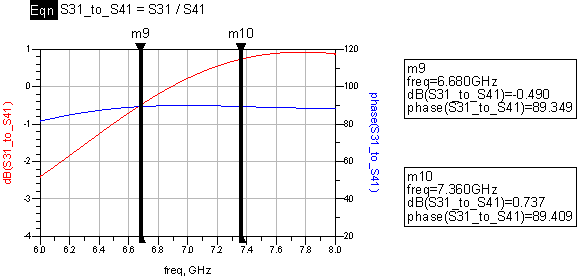
\includegraphics[width=\textwidth]{branch_line_coupler_MLIN_data_2_S31_to_S41_response_ripple.pdf}
        \caption{}
        \label{fig:branch_line_coupler_MLIN_data_2_S31_to_S41_response_ripple}
    \end{subfigure}
    \vfill
    \begin{subfigure}[b]{0.6\textwidth}
        \centering
        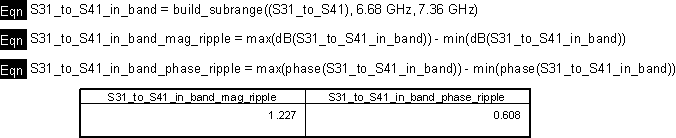
\includegraphics[width=\textwidth]{branch_line_coupler_MLIN_data_2_S31_to_S41_response_ripple_table.pdf}
        \caption{}
        \label{fig:branch_line_coupler_MLIN_data_2_S31_to_S41_response_ripple_table}
    \end{subfigure}
    \caption{
        Неравномерность рабочего затухания и переходного ослабления:
        a) графическое представление;
        б) табличное представление
    }
    \label{fig:branch_line_coupler_MLIN_data_2_response_ripple}
\end{figure}

\subsection{Модель на топологическом уровне}

Скопируем схему в микрополосковом исполнении в новую ячейку. Сделаем её двухуровневой, перенеся во внутренний уровень все полосковые устройства. Сделать это можно по команде Edit\textrightarrow Component\textrightarrow Create Hierarchy.

В результате получим схему верхнего уровня (Рис. \ref{fig:branch_line_coupler_EM_schematic}) и схему нижнего уровня (Рис. \ref{fig:branch_line_coupler_EM_inner_schematic}).

\begin{figure}[!ht]
    \centering
    \begin{subfigure}[b]{0.45\textwidth}
        \centering
        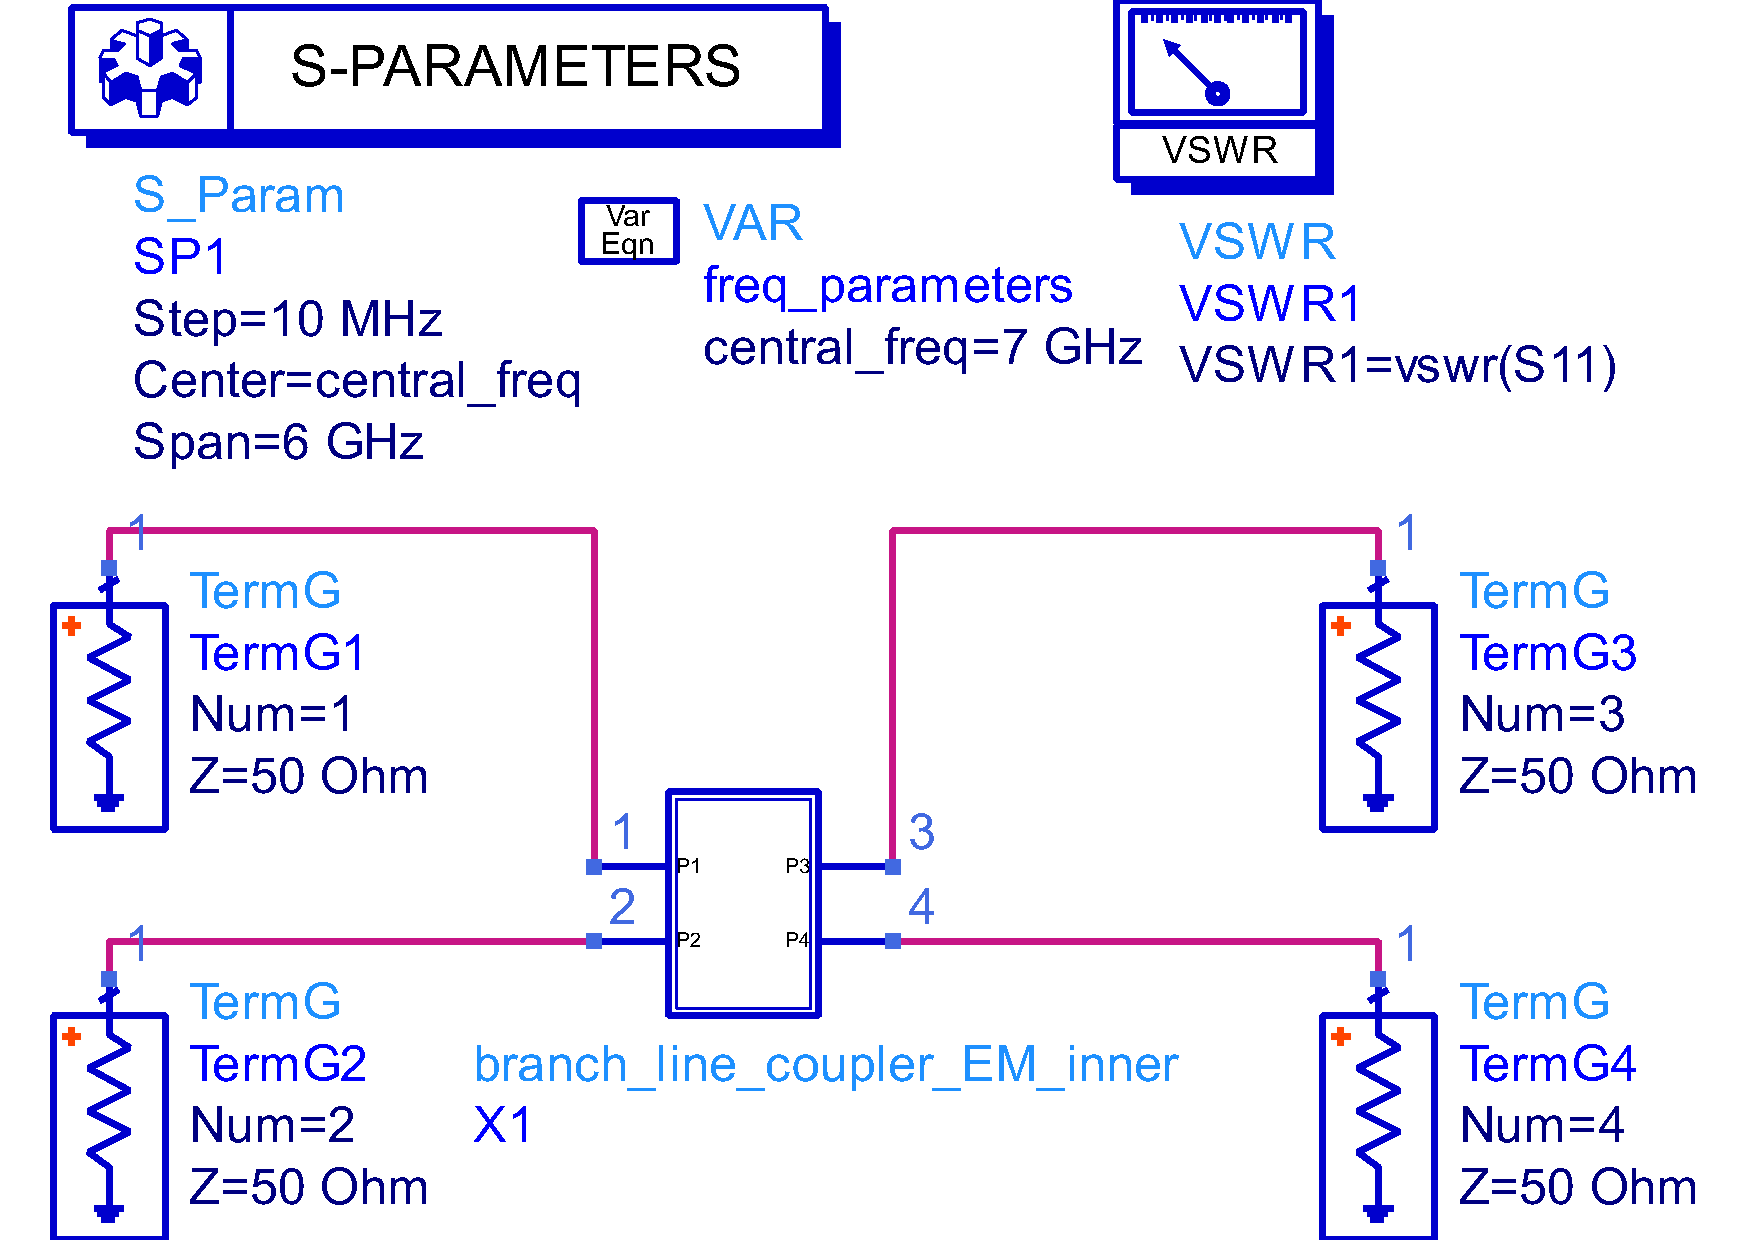
\includegraphics[width=\textwidth]{branch_line_coupler_EM_schematic_1.pdf}
        \caption{}
        \label{fig:branch_line_coupler_EM_schematic}
    \end{subfigure}
    \hfill
    \begin{subfigure}[b]{0.45\textwidth}
        \centering
        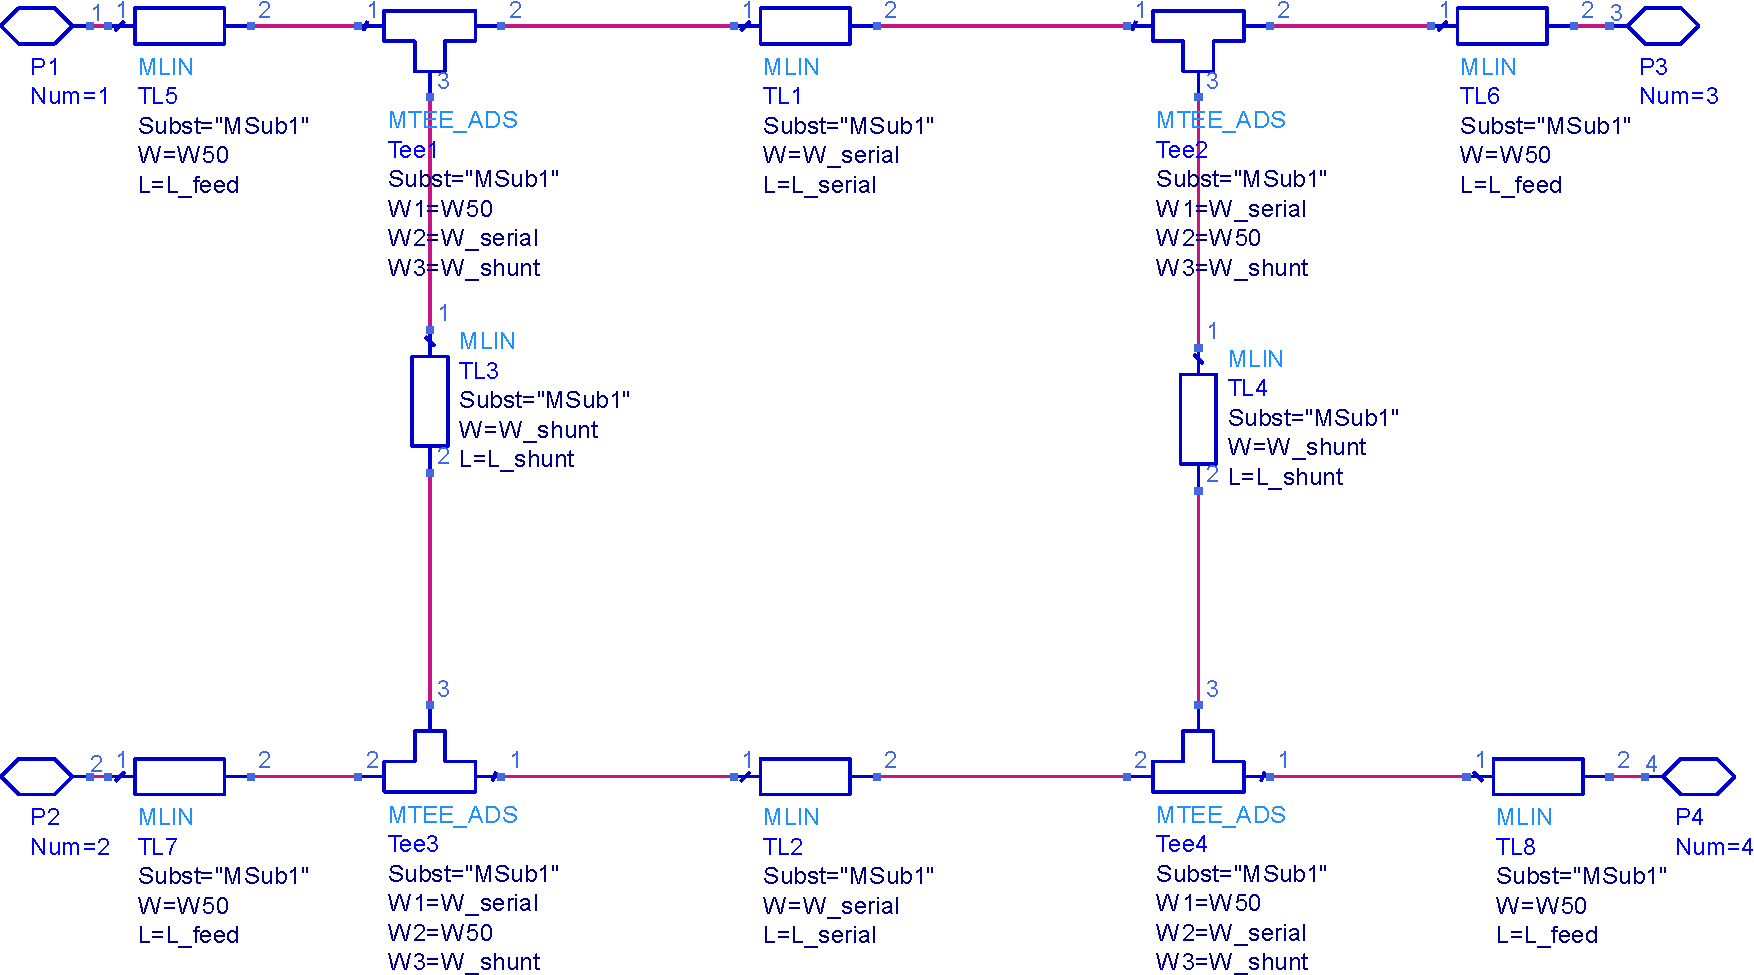
\includegraphics[width=\textwidth]{branch_line_coupler_EM_inner_schematic_1.pdf}
        \caption{}
        \label{fig:branch_line_coupler_EM_inner_schematic}
    \end{subfigure}
    \caption{
        Моделируемая схема на топологическом уровне:
        a) внешнаяя схема;
        б) внутренняя схема
    }
    \label{fig:branch_line_coupler_EM_schematics}
\end{figure}

Перейдём в схему нижнего уровня. Для получения топологического представления воспользуемся функцией Layout\textrightarrow Generate/Update Layout.
Топологическое представление создано верно (Рис. \ref{fig:branch_line_coupler_layout_check}).

\begin{figure}[!ht]
    \centering
    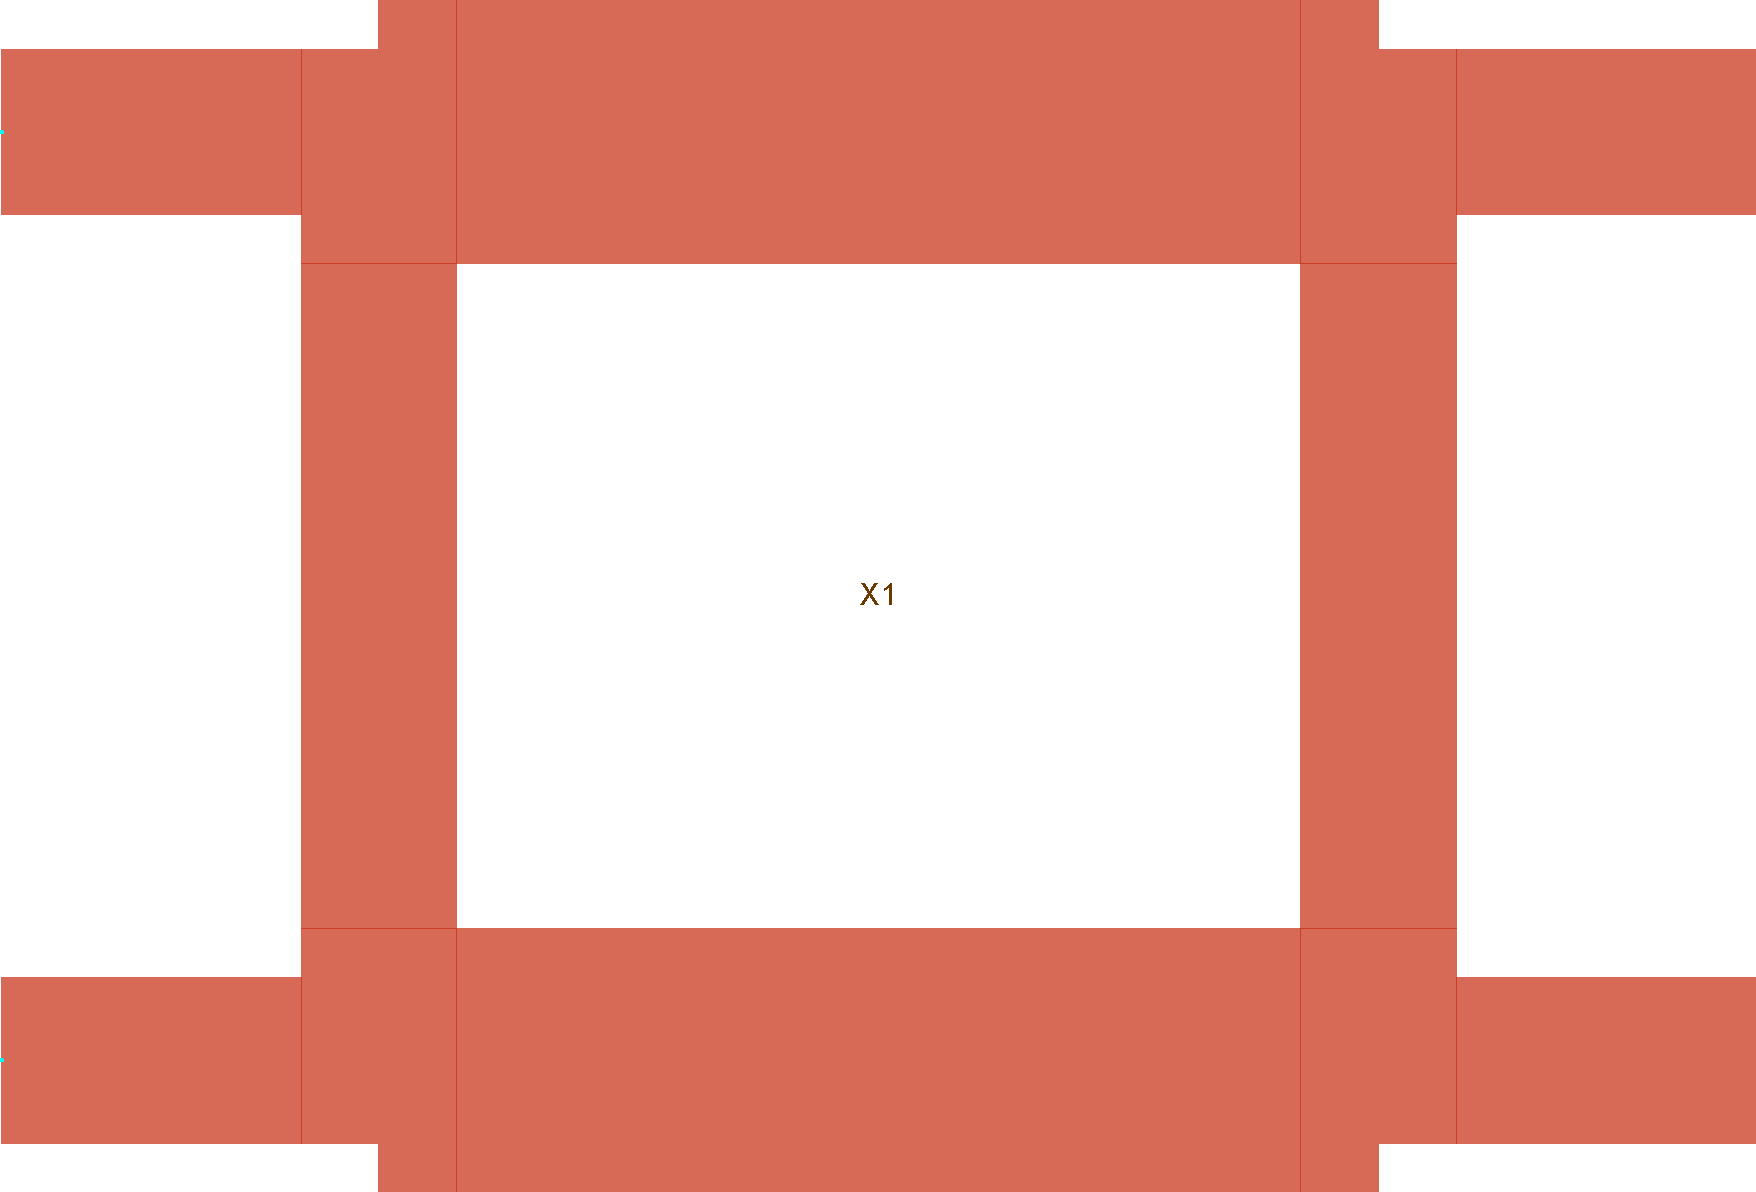
\includegraphics[width=0.6\textwidth]{branch_line_coupler_layout_check.pdf}
    \caption{Проверка топологического представления}
    \label{fig:branch_line_coupler_layout_check}
\end{figure}

Перейдём в окно File\textrightarrow Customize Pcell.
Сделаем схему параметризуемой, выбрав в выпадающем списке тип Parameterized sub network Pcell.
Также убедимся в том, что выставлены галочки напротив Support non-90 degree rotation и Support unit and database resolution for ADS 2015 and older.

В окне File\textrightarrow Cell Parameters определим параметры $W_{50}$, $L_\text{feed}$, $L_\text{shunt}$, $L_\text{serial}$.

Для EM-моделирования создадим сущность emSetup.
Это можно сделать в окне EM\textrightarrow Simulation Setting.
Определим параметры в соответствии с требованиями.

Запустим моделирование S-параметров нажатием кнопки Simulate.
В результате на топологии появится сетка (Рис. \ref{fig:branch_line_coupler_layout_sparam}).

\begin{figure}
    \centering
    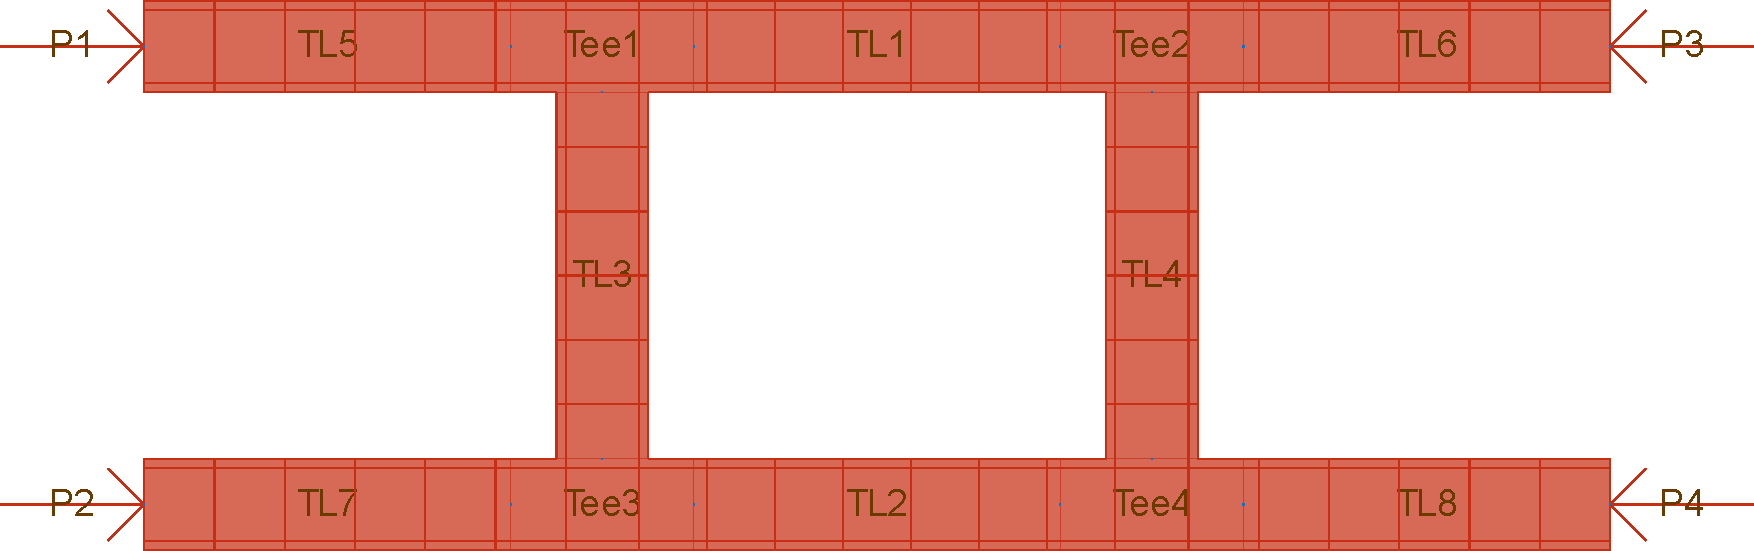
\includegraphics[width=0.6\textwidth]{branch_line_coupler_layout_sparam.pdf}
    \caption{Сетка на топологическом представлении после проведения EM-моделирования}
    \label{fig:branch_line_coupler_layout_sparam}
\end{figure}

Из окна emSetup можно обновить отображение элемента на схеме.
Сделаем так, чтоб оно подгружалось из топологии (Рис. \ref{fig:branch_line_coupler_EM_symbol}).
\begin{figure}
    \centering
    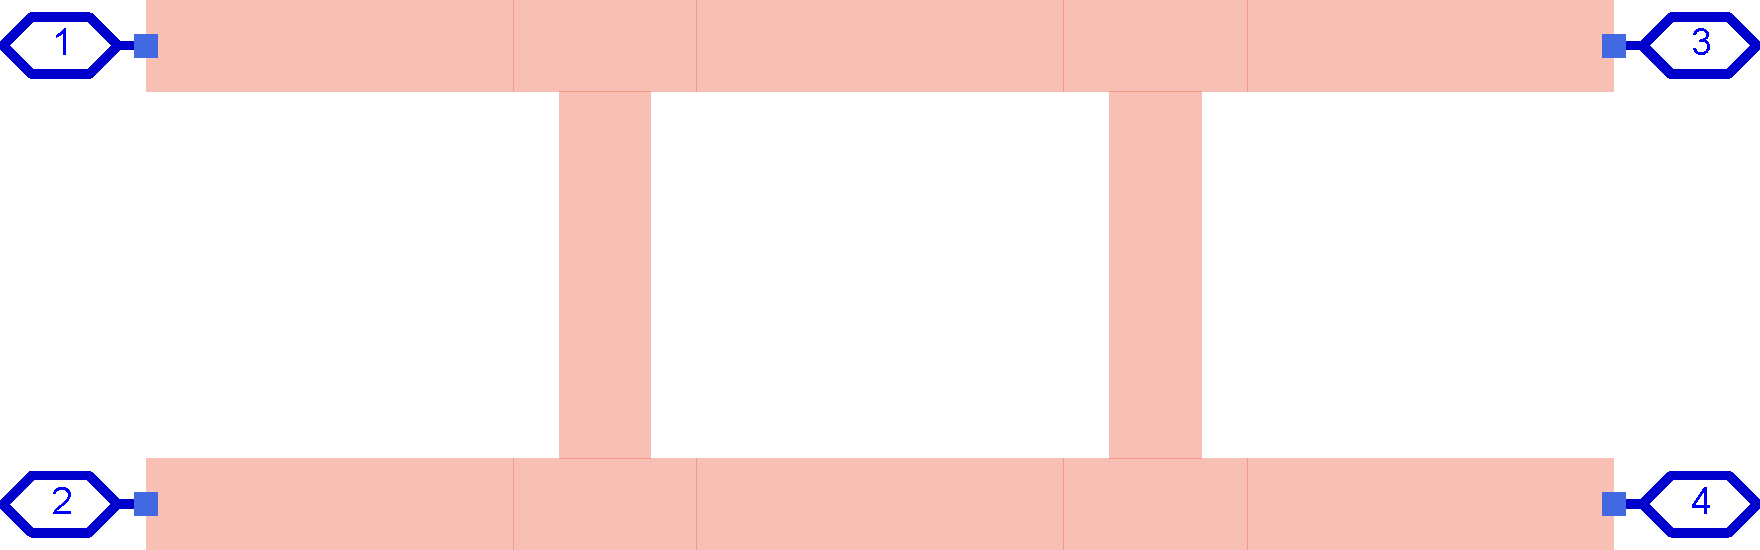
\includegraphics[width=0.6\textwidth]{branch_line_coupler_EM_symbol.pdf}
    \caption{Обновлённый символ}
    \label{fig:branch_line_coupler_EM_symbol}
\end{figure}
В итоге схема приобретёт вид как на рис. \ref{fig:branch_line_coupler_EM_schematic_2}.
\begin{figure}
    \centering
    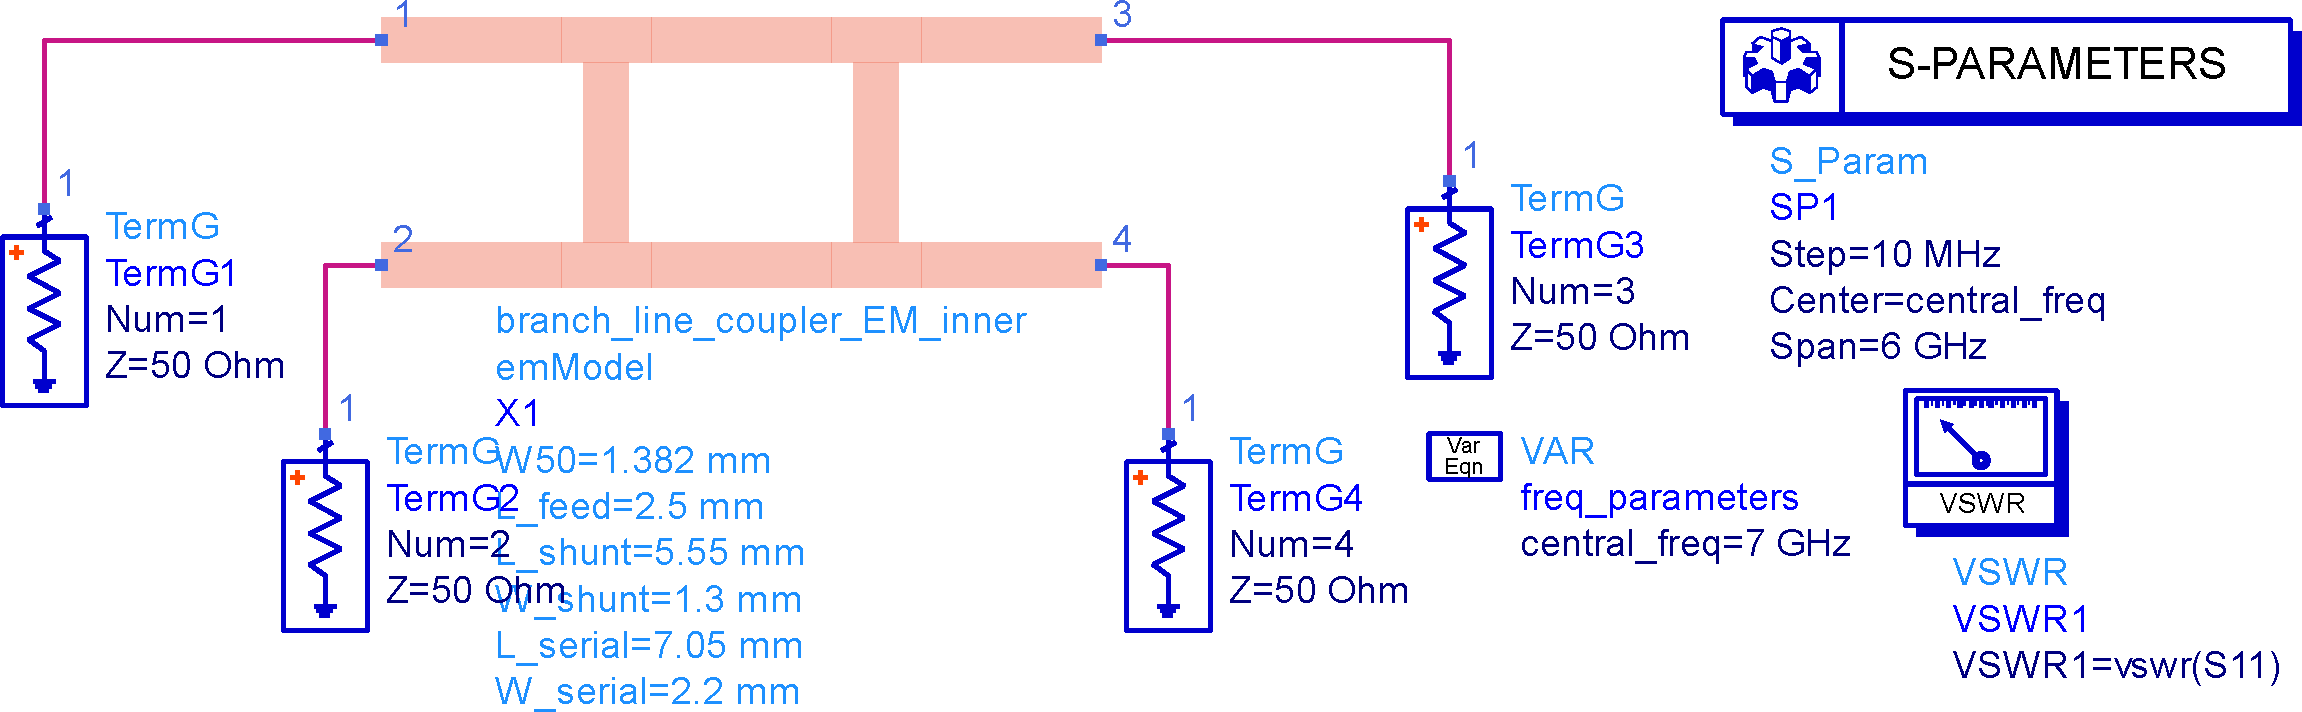
\includegraphics[width=0.8\textwidth]{branch_line_coupler_EM_schematic_2.pdf}
    \caption{Итоговый вид схемы}
    \label{fig:branch_line_coupler_EM_schematic_2}
\end{figure}

Запустим моделирование и отобразим частотные характеристики (Рис. \ref{fig:branch_line_coupler_EM_data_1}).

\begin{figure}[!ht]
    \centering
    \begin{subfigure}[b]{0.45\textwidth}
        \centering
        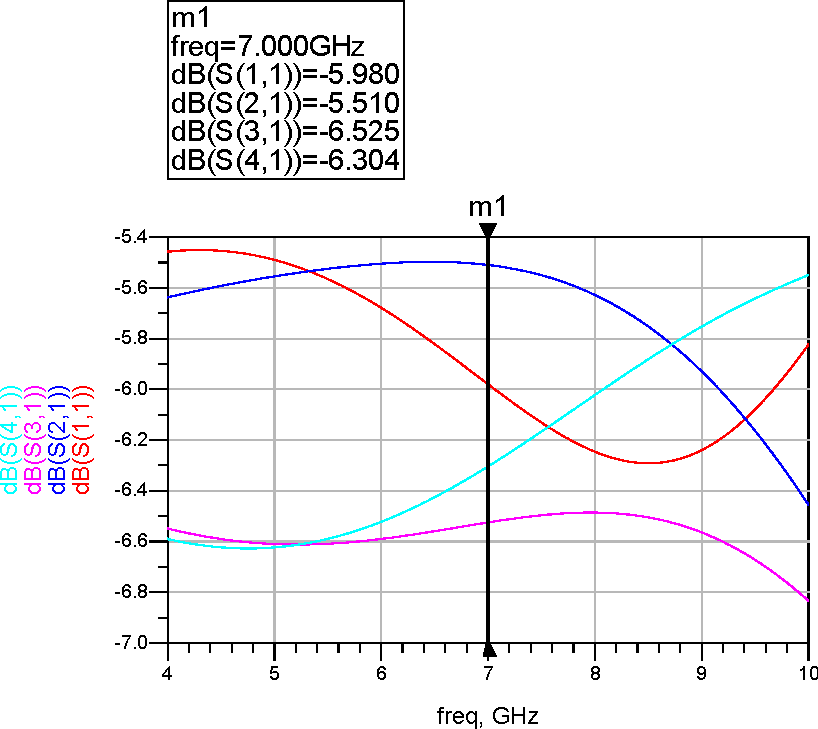
\includegraphics[width=\textwidth]{branch_line_coupler_EM_data_1_freq_response.pdf}
        \caption{}
        \label{fig:branch_line_coupler_EM_data_1_freq_response}
    \end{subfigure}
    \hfill
    \begin{subfigure}[b]{0.45\textwidth}
        \centering
        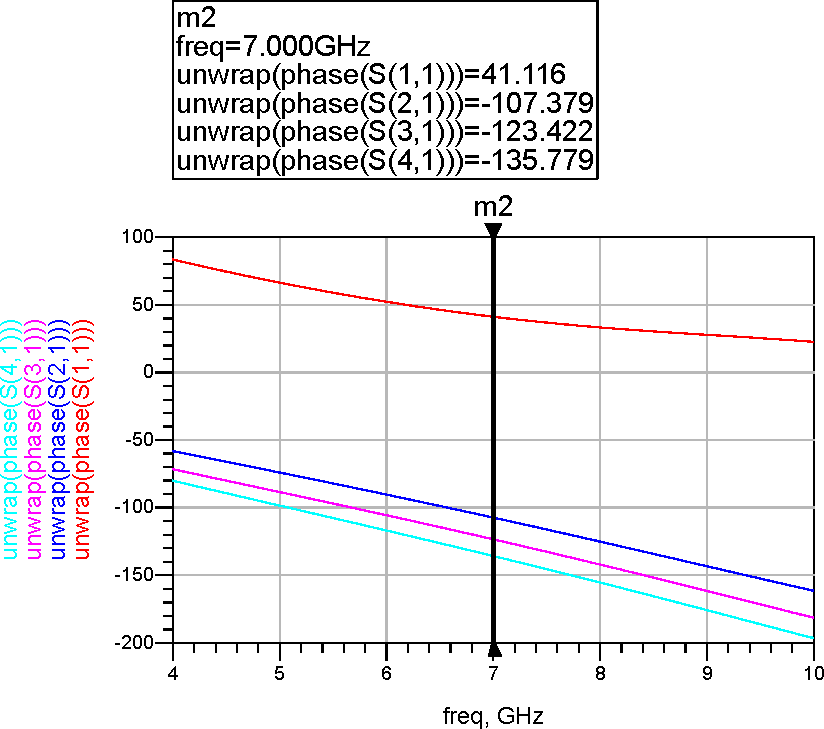
\includegraphics[width=\textwidth]{branch_line_coupler_EM_data_1_phase_response.pdf}
        \caption{}
        \label{fig:branch_line_coupler_EM_data_1_phase_response}
    \end{subfigure}
    \caption{
        Частотные характеристики моделируемой схемы в топологическом представлении:
        а) АЧХ;
        б) ФЧХ
    }
    \label{fig:branch_line_coupler_EM_data_1}
\end{figure}

Из графиков видно, что частоты сильно уплыли. Поправим это подбором параметров. Итоговые значения можно увидеть на рис. \ref{fig:branch_line_coupler_EM_schematic_3} а результаты моделирования на рис. \ref{fig:branch_line_coupler_EM_data_2}.

\begin{figure}[!ht]
    \centering
    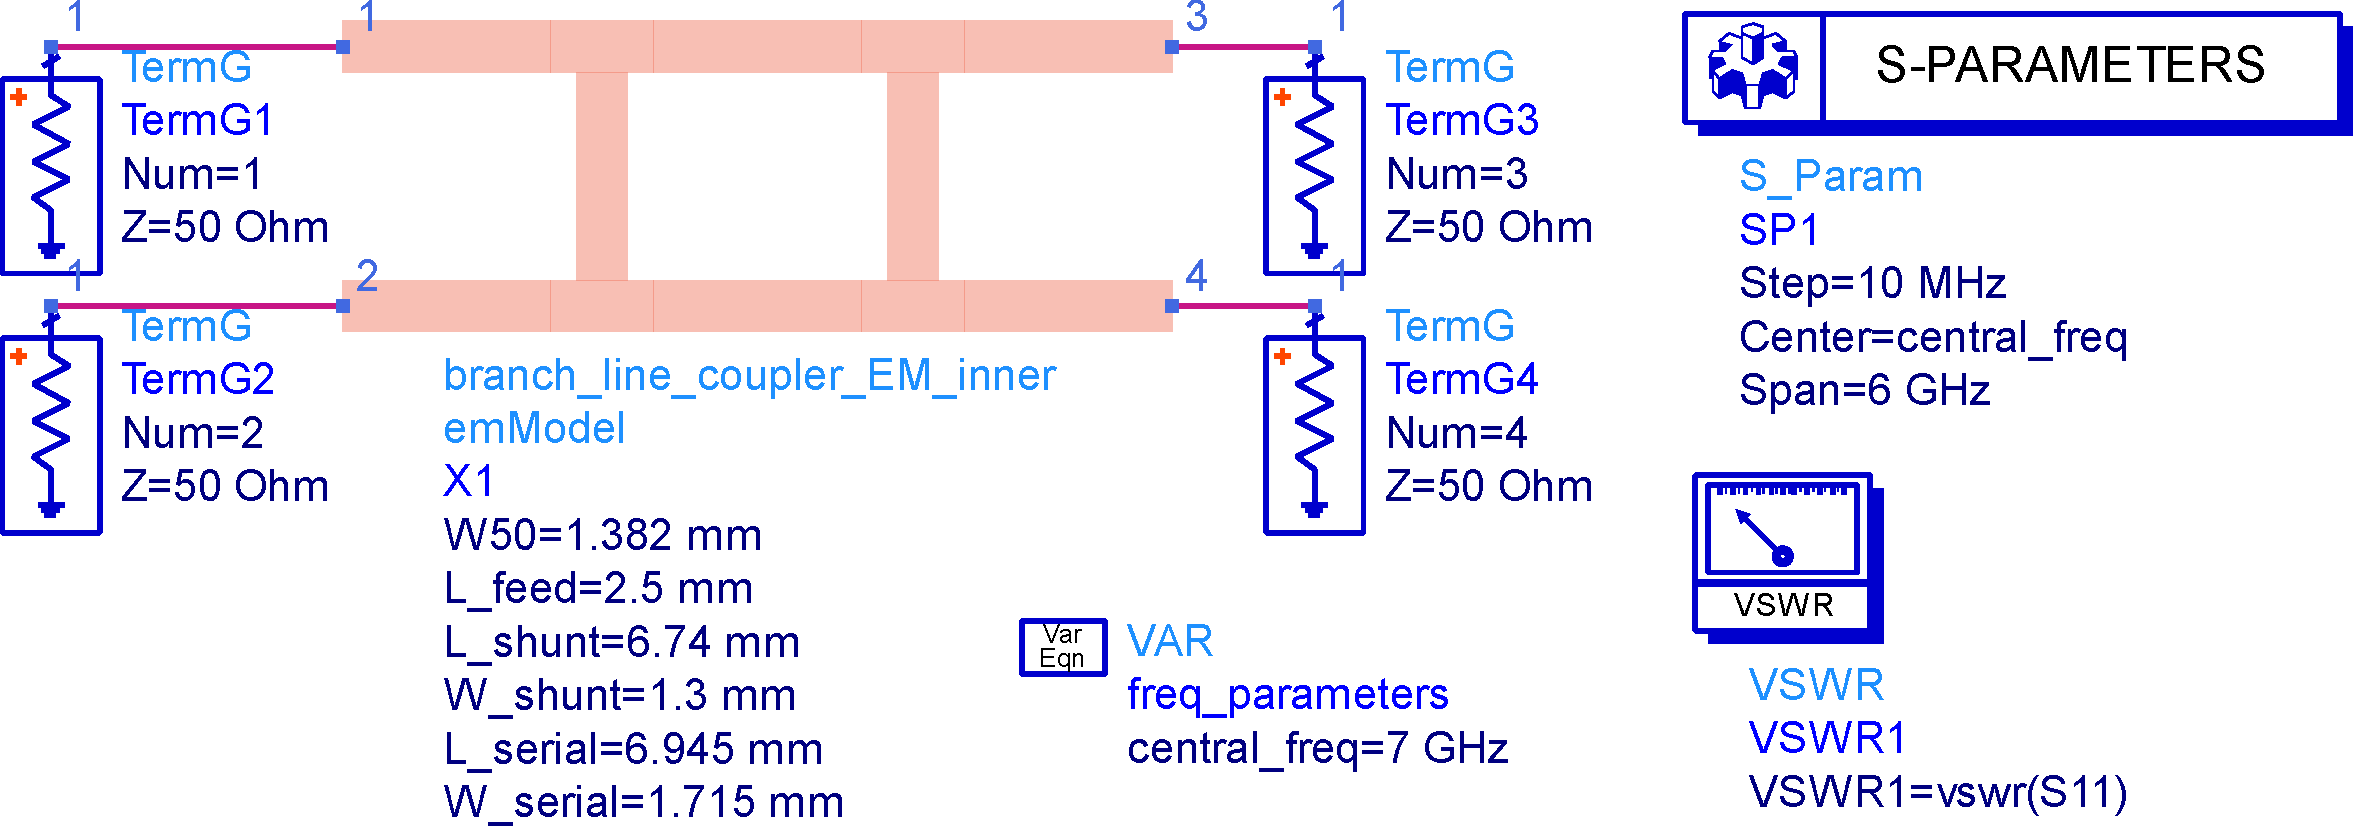
\includegraphics[width=0.8\textwidth]{branch_line_coupler_EM_schematic_3.pdf}
    \caption{Схема после подбора параметров}
    \label{fig:branch_line_coupler_EM_schematic_3}
\end{figure}

\begin{figure}[!ht]
    \centering
    \begin{subfigure}[b]{0.45\textwidth}
        \centering
        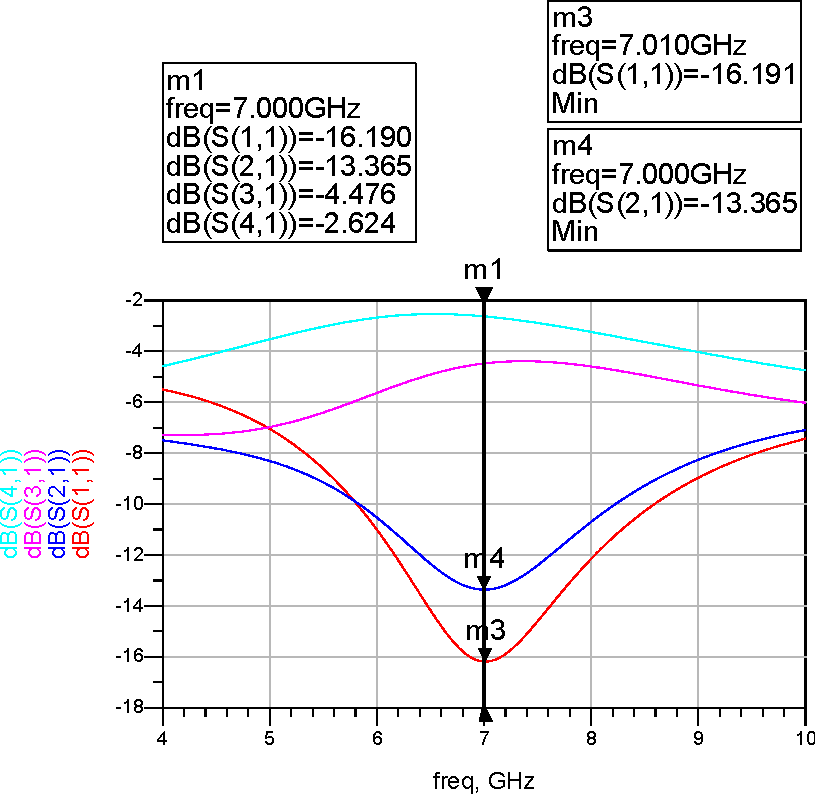
\includegraphics[width=\textwidth]{branch_line_coupler_EM_data_2_freq_response.pdf}
        \caption{}
        \label{fig:branch_line_coupler_EM_data_2_freq_response}
    \end{subfigure}
    \hfill
    \begin{subfigure}[b]{0.45\textwidth}
        \centering
        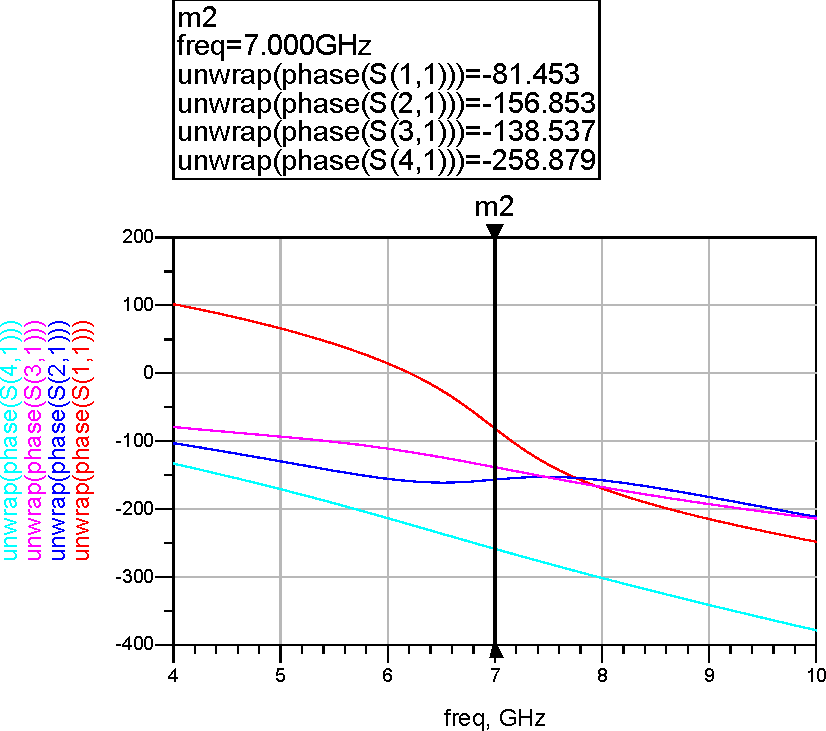
\includegraphics[width=\textwidth]{branch_line_coupler_EM_data_2_phase_response.pdf}
        \caption{}
        \label{fig:branch_line_coupler_EM_data_2_phase_response}
    \end{subfigure}
    \caption{
        Частотные характеристики моделируемой схемы в топологическом представлении после подбора параметров:
        а) АЧХ;
        б) ФЧХ
    }
    \label{fig:branch_line_coupler_EM_data_2}
\end{figure}
